\input{../../../header.tex}


\begin{document}
	\begin{titlepage}
		\centering
		\includegraphics[width=0.50\textwidth]{/home/eric/Uni/htw_logo.png}\par\vspace{1cm}
		{\scshape\LARGE HTW Dresden \par}
		\vspace{2cm}
		{\huge\bfseries Internet Technologien II \par}
		\vspace{2cm}
		{\Large\itshape Dokumentaion zur Belegaufgabe von\par Eric \textsc{S.} \par}
		\vfill
		s73952 \ret
		\vfill
		{13.01.2018}
	\end{titlepage}
\newpage \tableofcontents \newpage


\section{Einführung}
\subsection{Client}
Ergänzen Sie die Klasse Client entsprechend der in der Projektbeschreibung und den Kommentaren im Quelltext gegebenen Hinweisen.
\subsection{Server}
Ergänzen Sie die Klasse RTPpacket entsprechend der in der Projektbeschreibung und den Kommentaren im Quelltext gegebenen Hinweisen.
\subsection{RTSP-Methoden}
Ergänzen Sie die RTSP-Methoden OPTIONS und DESCRIBE anhand der Beispiele aus RFC 2326 und RFC 2327. Es ist ausreichend, sich bei DESCRIBE auf das Beispielvideo zu beziehen.
\subsection{Simulation von Paketverlusten}
Simulieren Sie Paketverluste und eine variable Verzögerung im Netz, indem Sie am Sender eine wahlweise Unterdrückung von zu sendenden Paketen vornehmen. Diese Unterdrückung von Paketen sollte zufällig und mit einstellbarer Paketverlustwahrscheinlichkeit über das GUI erfolgen. Beispiel: der Wert 0,1 bedeutet, es werden im Mittel 10% der zu übertragenen Pakete unterdrückt.
\subsection{Anzeige von Statistiken am Client}

Um die simulierten Netzwerkeigenschaften prüfen zu können und die Leistungsfähigkeit der später zu integrierenden Fehlerschutzcodes einschätzen zu können, ist eine Statistikanzeige notwendig. Folgende Werte sollten mindestens am Client angezeigt werden:
\begin{enumerate}
	\item Anzahl erhaltener/verlorener Medienpakete + prozentuale Angabe
	\item Anzahl korrigierter/unkorrigierbarer Medienpakete
	\item Die Anzeige sollte bis zum Ende des Videos sekündlich aktualisiert werden und dann auf dem Gesamtstand stehen bleiben.
\end{enumerate}

Mit dem ersten Punkt kann die Qualität der Verbindung eingeschätzt werden und mit dem zweiten Punkt die Leistungsfähigkeit des FEC-Verfahrens. Machen Sie sich Gedanken über weitere zu überwachende Parameter.
\subsection{Implementierung des FEC-Schutzes}
Implementieren Sie einen FEC-Schutz mittels Parity-Check-Code (XOR mit k = 2...20, p = 1). Der Parameter sollte am Server einstellbar sein (GUI / Kommandozeile). Um die Gruppengröße dem Client mitzuteilen gibt es mehrere Möglichkeiten. Der Parameter könnte explizit in einem FEC-Header mitgeteilt werden oder der Client trackt den Wert anhand der Abfolge der Pakete.

Der Server mit FEC-Schutz soll kompatibel zu Clients ohne FEC-Verfahren sein! Nutzen Sie dazu das Feld Payloadtype des RTP-Headers (PT=127 für FEC-Pakete). Sie können sich bei der Implementierung an RFC 5109 orientieren, dies ist aber keine Pflicht. Sie sollten aber das Dokument zumindest lesen.

Implementierung Sie FEC über nachfolgende Schritte:
\begin{enumerate}
	\item Nutzung einer separaten Klasse FECpacket für das FEC-Handling für Sender und Empfänger, siehe Architekur	
	\item Serverseitige Implementierung des XOR-FEC. Nach Auswertung des PT (26) sollte der Client nach wir vor regulär funktionieren.
	\item Entwurf der Architektur der Paket- und Bildverarbeitung im Client
	\item Eingangspuffer im Client implementieren (Größe ca. 1-2 s)
	\item FEC-Korrektur im Client implementieren
\end{enumerate}

Ändern Sie die vorhandenen Klassen nur soweit nötig. Halten Sie die Struktur einfach und überschaubar. Nutzen Sie Threads nur wenn dies notwendig ist und Sie die Nebenwirkungen (Blockierungen, Race-Condition) kennen. Bei einer durchdachten Implementierung benötigen Sie keine Threads.

\ret
Die detaillierte Aufgabenstellung entnehmen Sie bitte hier:\ret \url{https://github.com/HTWDD-RN/RTSP-Streaming/blob/master/Aufgabenstellung.md}

\section{Funktionsweise}
Um die Software zu starten muss es vorerst kompiliert werden. Dafür muss nur das SHELL-Skript im \textit{src}-Ordner \textit{./makefile} ausgeführt werden. Dies ist nur möglich, wenn auf dem zu verwendeten Rechner Java SDK installiert ist.\ret
Um den Server beziehungsweise den Client zu starten führt man das SHELL-Skript \textit{./run\_server} bzw. \textit{./run\_client} aus. Der Port für den Client und den Server ist Standard gemäß auf \textit{3333} eingestellt. Das Programm ist nun bereit.
\subsection{Server}
Der Server dient als Sender der Datenpakete. Es ist möglich, den Server ohne einen Port zu starten. Sollte dies der Fall sein, wird der Nutzer aufgefordert einen Port händisch einzutragen. \ret
Im Server wird immer ein Datenpaket und ein FEC-Paket erstellt. Je nachdem wie das k eingestellt wurde, werden diese Pakete als Gruppe der Größe k versendet. \ret
Wenn der Nutzer den Button \textit{TEARDOWN} gedrückt hat, wird dies abgefangen und die Session sowie das Programm beendet.


\subsection{Client}
Der Client dient als Empfänger der Daten (des Filmes). Es ist möglich, den Client ohne einen Server, Port und Film zu starten. Sollte dies der Fall sein, wird der Nutzer aufgefordert einen Server, Port und Film händisch einzutragen. \\
Die Datenpakete werden entgegengenommen und dem Nutzer jeweils graphisch dargestellt. Sollte ein Paket fehlen, was Anhand der fehlenden Paketnummer/Sequenznummer geprüft wird, wird versucht das fehlende Paket mittels FEC wieder zu restaurieren. Dazu werden alle anderen Bilder in der jeweiligen Gruppe herangezogen. Sollte dies nicht funktionieren, wird das in der Konsole dokumentiert. \ret
Wenn der Nutzer den Button \textit{TEARDOWN} drückt, wird dies an den Server übermittelt und die Session und das Programm beendet. \ret
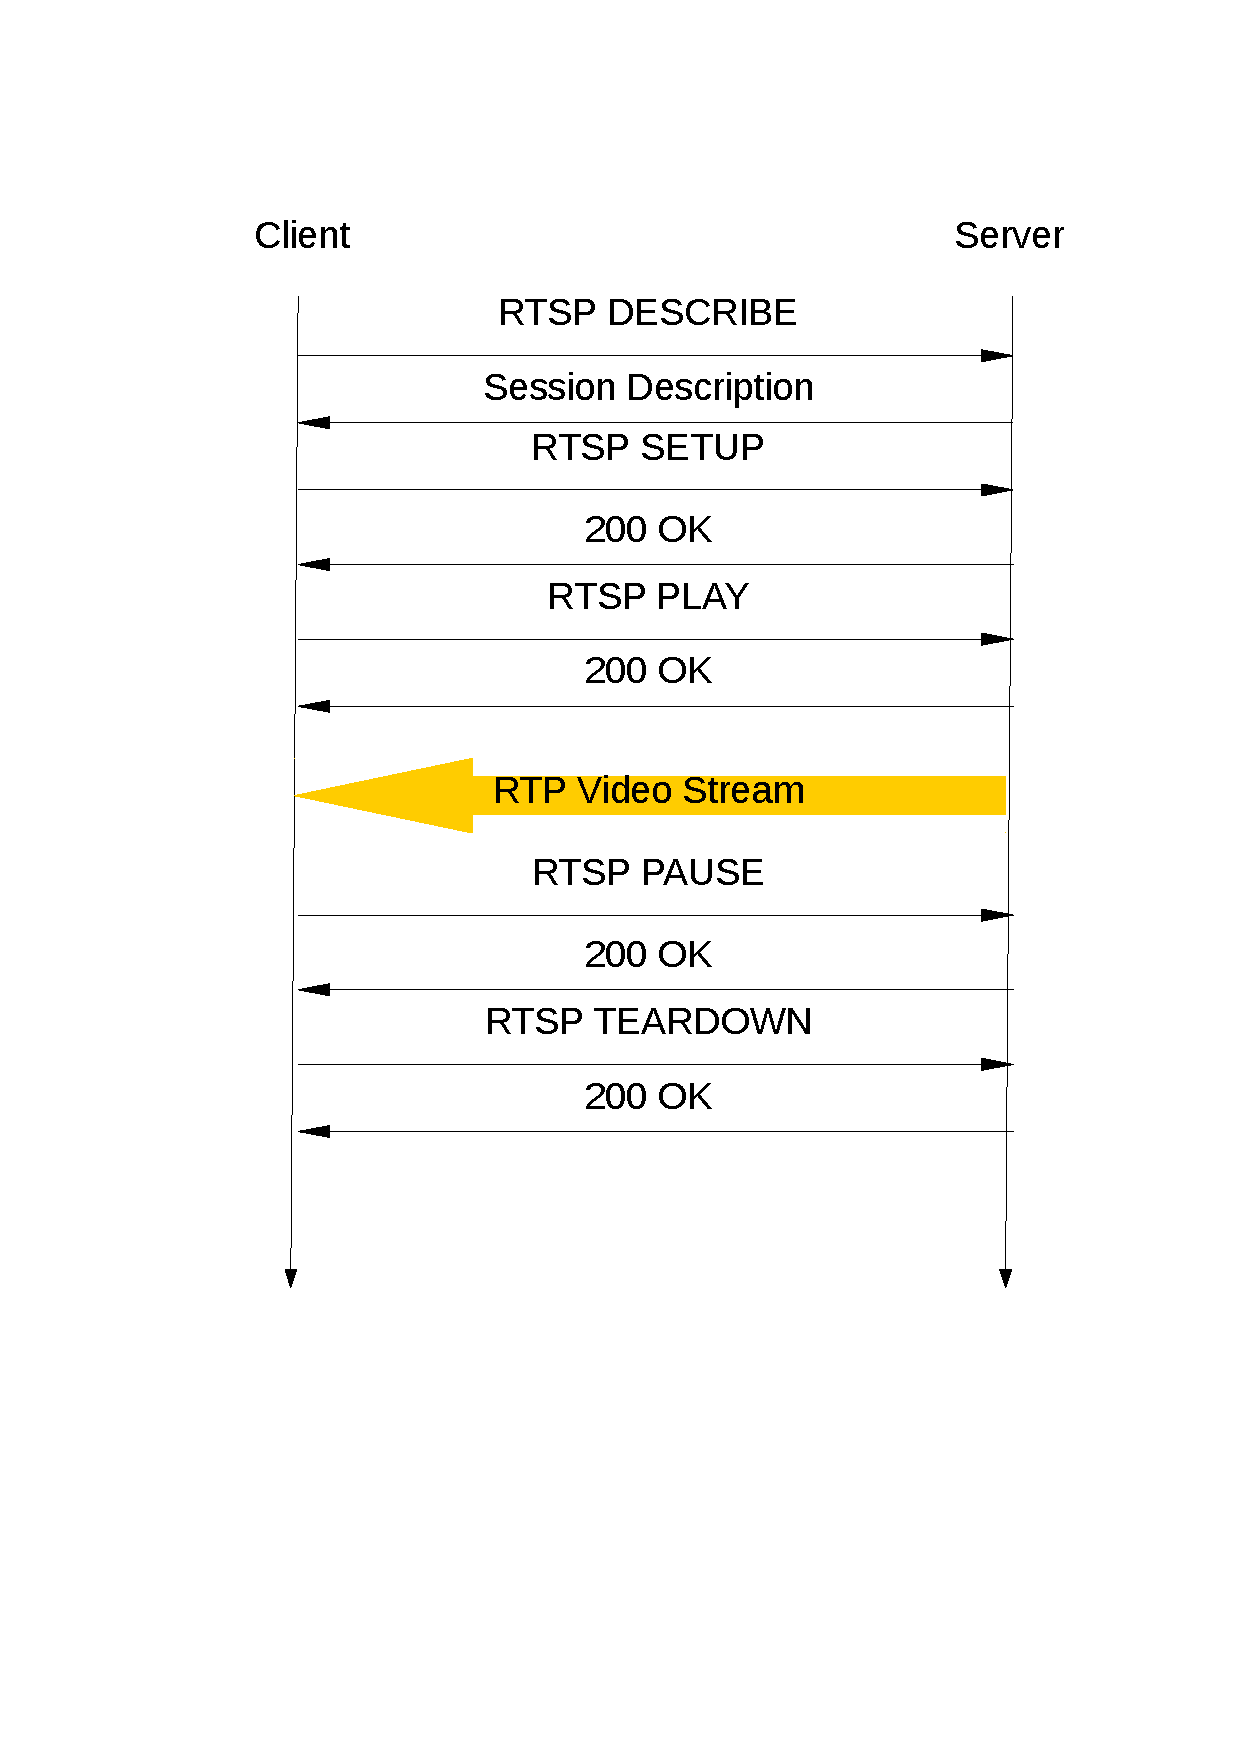
\includegraphics[scale=0.45]{handshake01.pdf} \newline

\subsection{FEC}
Vorwärtsfehlerkorrektur (Englisch 'forward error correction', kurz FEC) ist eine Technik, die dazu dient, die Fehlerrate bei der Speicherung oder der Übertragung digitaler Daten zu senken, und stellt ein Fehlerkorrekturverfahren dar. Der Server kodiert die zu übertragenden Daten in redundanter Weise, sodass der Client Übertragungsfehler ohne Rückfrage vom Server erkennen und korrigieren kann.

\subsubsection*{FEC Manager}
Der grundlegende Ablauf ist wie folgt:
\begin{itemize}
	\item Datenpakete buffern
	\item Server erstellt FEC Pakete
	\item Client korrigiert Datenpakete
\end{itemize}
Der Buffer für die Datenpakete hat jeweils eine feste Größe.

\subsubsection*{Korrigieren von Datenpaketen}
Der Client kann in der Gruppe kaputte oder verlorene Datenpakete korrigieren. Um ein defektes Paket in einer Gruppe zu korrigieren, werden alle anderen Pakete in der Gruppe mit herangezogen. Danach werden alle Markierungen in dem Buffer gelöscht und der Index wird weiter geschaltet.
\section{Probleme}
Bei mir kam es zum Ende hin zu einigen Problemen. Die Implementation Forward Error Correction hat mich einiges an Zeit gekostet. Zudem musste ich hier viel debuggen um wirklich alle Fehler abzufangen und dem Code zu optimieren. Die Implementation zum einstellen der Gruppengröße habe ich leider nicht abschließen können. Das Prinzip ist mir aber klar. Mir ist oft der Server abgestürzt oder er sendete kein Bild mehr. Daher habe ich mich dann entschlossen in meinem Repository zwei Versionen zurück zu gehen, um überhaupt keine funktionierende Lösung abgeben zu können. 

\end{document}